\begin{table}[H]\centering\small
\begin{tabular}{@{}lrrrrr@{}}\toprule
Configuration & Accepted & Hosted seconds & Operations & Test runs & Actual cost \\ \midrule
U & 4/4 & 372.46 & 32 & 8 & Unknown \\
E & 4/4 & 275.35 & 33 & 8 & Unknown \\
E+ & 4/4 & 353.62 & 36 & 8 & Unknown \\
\bottomrule\end{tabular}
\caption{Observed frozen batches under the same 1,500-second/64-operation outer limits. Counts are successfully logged interface operations, not complete token telemetry. All final submissions meet their recorded budgets.}
\end{table}
The observed acceptance differences E--U and E+--E are both zero percentage points on these four missions. E's hosted batch is shorter than U's; E+ is longer than E's. These single observations are descriptive and cannot identify a reliable latency, hidden-compute or dollar-cost effect. U's eight test executions are all post-repair passes; E and E+ each retain four deliberately failing original-code regression runs before their passing repaired runs. Those reproduced defects are not failed final customer deliveries.
\begin{figure}[H]\centering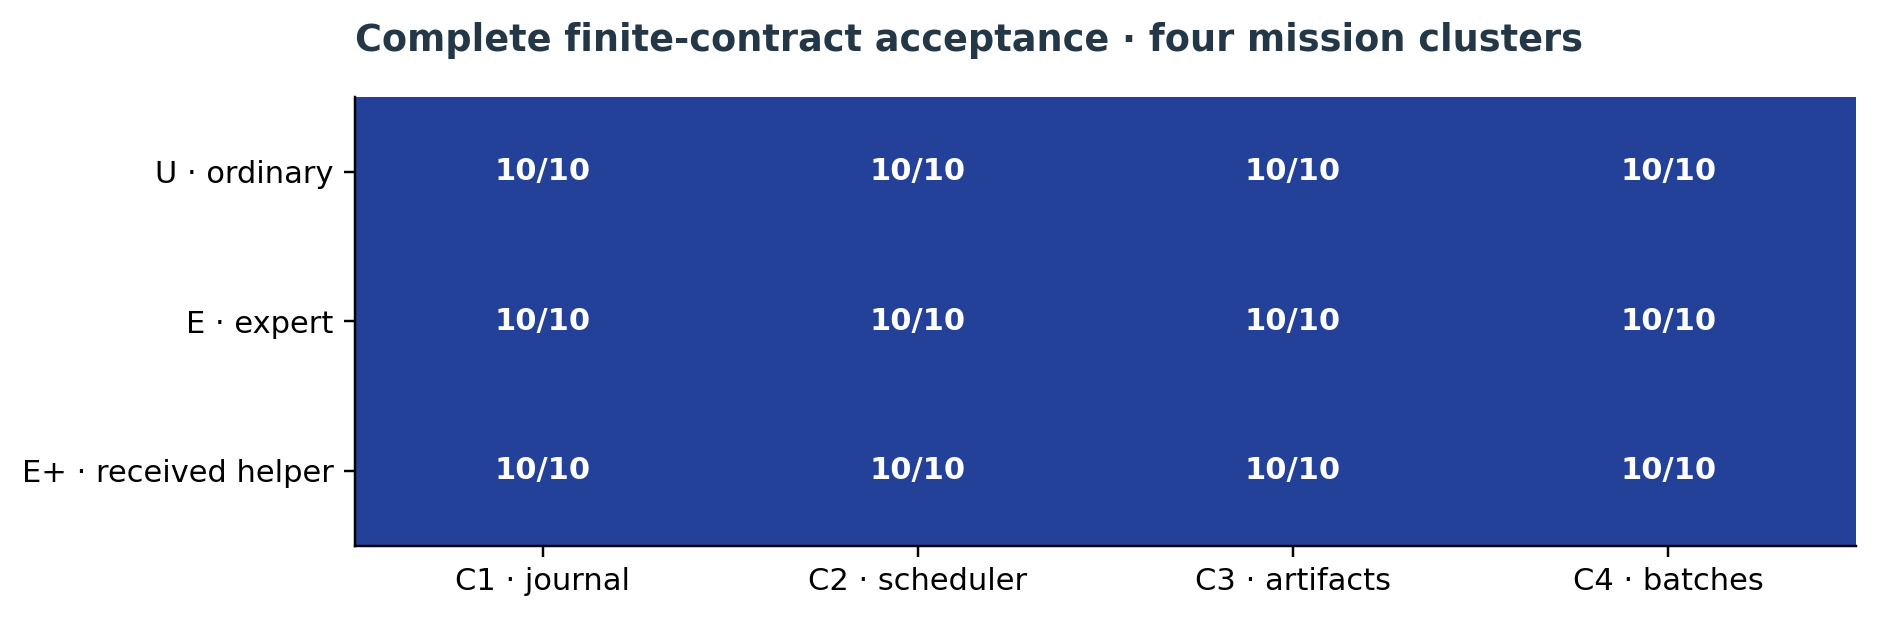
\includegraphics[width=0.95\linewidth]{figures/acceptance.png}\caption{All four complete contracts accept in each arm. The forty checks within an arm do not create forty independent tasks.}\end{figure}
\begin{figure}[H]\centering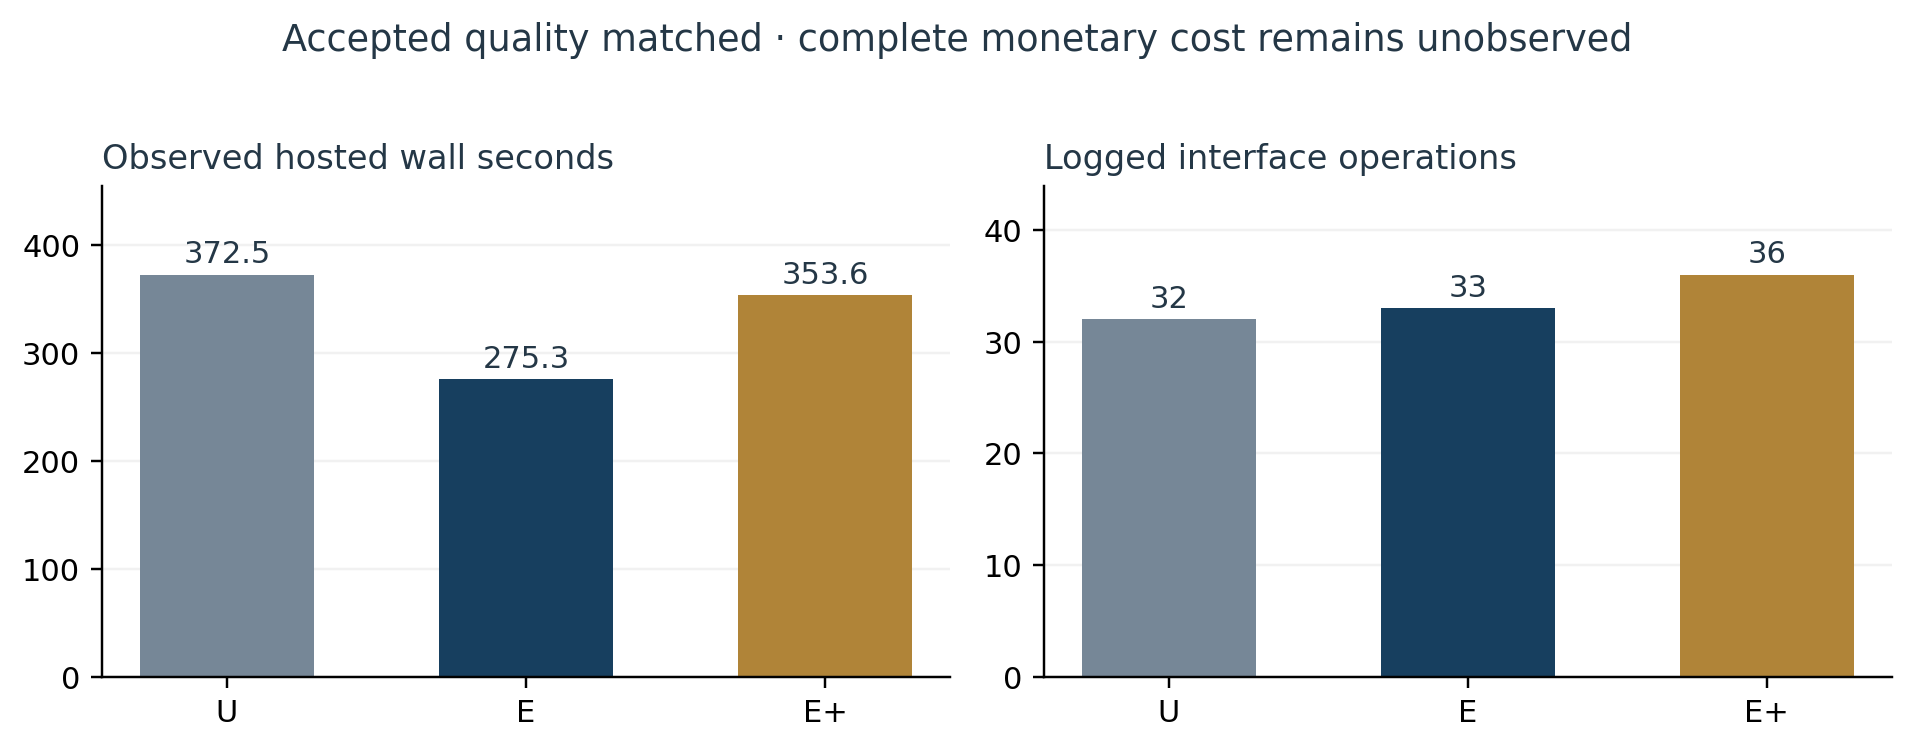
\includegraphics[width=0.95\linewidth]{figures/observed_resources.png}\caption{One hosted batch per arm. Model tokens, billing, provider scheduling and full research labor are not inferred from these bars.}\end{figure}
